\section{Theorie}

Das Emissionsspektrum von Atomen, in diesem Fall Cadmium, entsteht dadurch, dass gebundene Elektronen zwischen den diskreten Energieniveaus springen.
Zu jeder beobachteten Emissionslinie gehört die Differenz zweier Energieniveaus des Atoms.

\subsection{Magnetisches Moment von Elektronen und Atomen}

Aufgrund der Ladung und des Drehimpulses von Elektronen haben diese ein magnetisches Moment.
Das magnetische Moment eines Elektrons mit einer Drehimpulseinheit heißt Bohrsches Magneton $\mu_\text{B}$.
Zu den beiden Drehimpulsen des Elektrons, dem Bahndrehimpuls und dem Spin, lässt sich das magnetische Moment aufstellen:
\begin{align}
	\mu_\text{l} & = \mu_\text{B} \sqrt{l (l + 1)} \\
	\mu_\text{s} & = g_\text{S}\mu_\text{B} \sqrt{s (s + 1)}
\end{align}
Dabei ist $l$ die Bahndrehimpulsquantenzahl, $s$ die Spinquantenzahl und $g_\text{S}$ eine Korrekturkonstante, die ,,Landé-Faktor des Elektrons'' heißt.
Der Zahlenwert des Landé-Faktors des Elektrons ist etwa $2$.

Analog zu den magnetischen Momenten einzelner Elektronen gilt für das gesamte Atom näherungsweise:
\begin{align}
	\mu_\text{L} & = \mu_\text{B} \sqrt{L (L + 1)} \\
	\mu_\text{S} & = g_\text{S}\mu_\text{B} \sqrt{S (S + 1}
\end{align}
Dabei sind L und S die Quantenzahlen für das gesamte Atom.
Die Drehimpulse des Atoms sind die vektoriellen Summen der Elektronendrehimpulse.
Die Drehimpulse abgeschlossener Schalen heben sich auf.
Deswegen muss nur die Atomhülle betrachtet werden.

In einem Atom mit mehreren Elektronen treten Wechselwirkungen zwischen den beiden magnetischen Momenten und zwischen denen mehrerer Elektronen auf.
In einer Näherung für ein geringes äußeres Magnetfeld ist der Gesamtdrehimpuls die vektorielle Summe des Bahndrehimpulses und des Spins.
Dieser Fall heißt LS-Kopplung.
Zu dem Gesamtdrehimpuls $\vec{J}$ gehört die Drehimpulsquantenzahl $J$:
\begin{align}
	|\vec{J}| = \sqrt{J (J + 1)} \hbar
\end{align}
Die Drehimpulsquantenzahl ist der Index des Atomorbitals S, P, D, F, ...
Entsprechend gehört das Orbital S zu $J = 0$, P zu $J = 1$ und so weiter.

Aus den bisherigen Gleichungen und weiteren quantenmechanischen Überlegungen kann für das magnetische Moment $\mu$ der Elektronenhülle diese Gleichung aufgestellt werden:
\begin{align}
	\mu_\text{J} = g_\text{J} \mu_\text{B} \sqrt{J(J + 1)}
\end{align}
Dabei ist $g_\text{J}$ der Landé-Faktor des Atoms.
\begin{align}
	\label{landefaktor}
	g_\text{J} = \frac{3J(J+1) + S(S + 1) - L(L + 1)}{2 J(J + 1)}
\end{align}

\subsection{Atom im Magnetfeld}
Beim Anlegen eines homogenen äußeren Magnetfelds tritt der quantenmechanische Effekt der Richtungsquantelung ein.
Er besagt, dass der Winkel zwischen dem äußeren Magnetfeld $\vec{B}$ und dem magnetischen Moment des Atoms $\vec{\mu}$ so eingeschränkt ist, dass die Komponente der magnetischen Moments in Feldrichtung ein ganzzahliges Vielfaches von $g_\text{J} \mu_\text{B}$ ist.
Der zugehörige Faktor ist die Orientierungsquantenzahl $m$.
Ein weiteres quantenmechanisches Ergebnis ist, dass die zum Magnetfeld orthogonale Komponente des magnetischen Moments im zeitlichen Mittel verschwindet, $\mu_{\text{J}_\text{z}} = \mu_\text{J}$.
Folglich gilt:
\begin{align}
	\mu_\text{J} = -m g_\text{J} \mu_\text{B}
\end{align}
Da die Komponente höchstens so groß werden kann wie der gesamte Vektor, kann $m$ betragsmäßig höchstens so groß sein wie J.
Die möglichen Werte von $m$ sind folglich
\begin{align}
	m \in \{-J, -J + 1, ..., 0, 1, ..., J\}
\end{align}

Daraus lässt sich die magnetische Energie berechnen:
\begin{align}
	\label{emag}
	E_\text{mag} = - \vec{\mu}_\text{J} \cdot \vec{B} = m g_\text{J} \mu_\text{B} B
\end{align}
Ein Energieniveau in der Atomhülle mit der Energie $E_0$ wird im Magnetfeld in $2J + 1$ verschiedene Energien mit unterschiedlichen $m$ aufgespalten.

\subsection{Eigenschaften aufgespaltener Emissionslinien}
Aus der Lösung der Schrödingergleichung für die beiden Energieniveaus eines Übergangs ergibt sich, dass sich die Orientierungsquantenzahlen $m$ der beiden Energieniveaus gar nicht oder um $\pm1$ unterscheiden dürfen.
\begin{align}
	\Delta m \in \{-1, 0 , 1\}
\end{align}

Weiterhin lassen sich aus der Lösung der Schrödingergleichung Aussagen über die Polarisierung des abgestrahlten Lichts treffen.
Im Fall $\Delta m = 0$ sind ist das emittierte Licht linear polarisiert.
Die Polarisierung ist parallel zu $\vec{B}$.
Im Fall $\Delta m = \pm 1$ ist das Licht zirkular polarisiert.
Die Drehrichtung ist in beiden Fällen unterschiedlich.

Die zu $\Delta m = 0$ gehörigen Spektrallinien haben die gleiche Energie wie die ohne Magnetfeld beobachtete Linie.
Sie wird mit $\pi$ bezeichnet.
Die anderen Linien heißen $\sigma^+$ oder $\sigma^-$.

\subsection{Der normale Zeeman-Effekt}
Der normale Zeeman-Effekt ist der Sonderfall, bei dem der Elektronenspin nicht berücksichtigt wird.
\begin{align}
	S = 0, \quad \quad J = L
\end{align}
In diesem Fall vereinfacht sich der Landé-Faktor \eqref{landefaktor} zu
\begin{align}
	g_\text{J} = 1.
\end{align}
Folglich ist die magnetische Energie der Elektronenhülle \eqref{emag} nicht mehr von den Quantenzahlen $S$, $L$ und $J$ abhängig.
Die Energie eines Übergangs ist nur noch eine Funktion von $\Delta m$ und es sind genau drei Linien zu beobachten.
Für die Energie der beobachteten Spektrallinien gilt:
\begin{align}
	E = E_0 + \Delta E_\text{mag} =  E_0 + \Delta m \mu_\text{B} B
\end{align}
Dabei ist $E_0$ die Energie der Spektrallinie, die ohne Magnetfeld beobachtet wird.

\subsection{Der anormale Zeeman-Effekt}
Lässt man die Einschränkung $S = 0$ fallen, hängt die Energiedifferenz der Übergänge von den Landé-Faktoren der beteiligten Energieniveaus und somit von deren Quantenzahlen $S$, $L$ und $J$ ab.

Die Energie einer Spektrallinie ist
\begin{align}
	E &= E_0 + \Delta E_\text{mag} \\
	&= E_0 + \mu_\text{B} B \left(m_1 g_\text{J,1} - m_2 g_\text{J,2} \right) \\
	&= E_0 + \mu_\text{B} B \Delta mg.
\end{align}
Dabei ist $E_0$ die Energie der Spektrallinie, die ohne Magnetfeld beobachtet wird.

\subsection{Termschema der roten und blauen Linien des Cadmium-Spektrums}
\begin{figure}
	\centering
	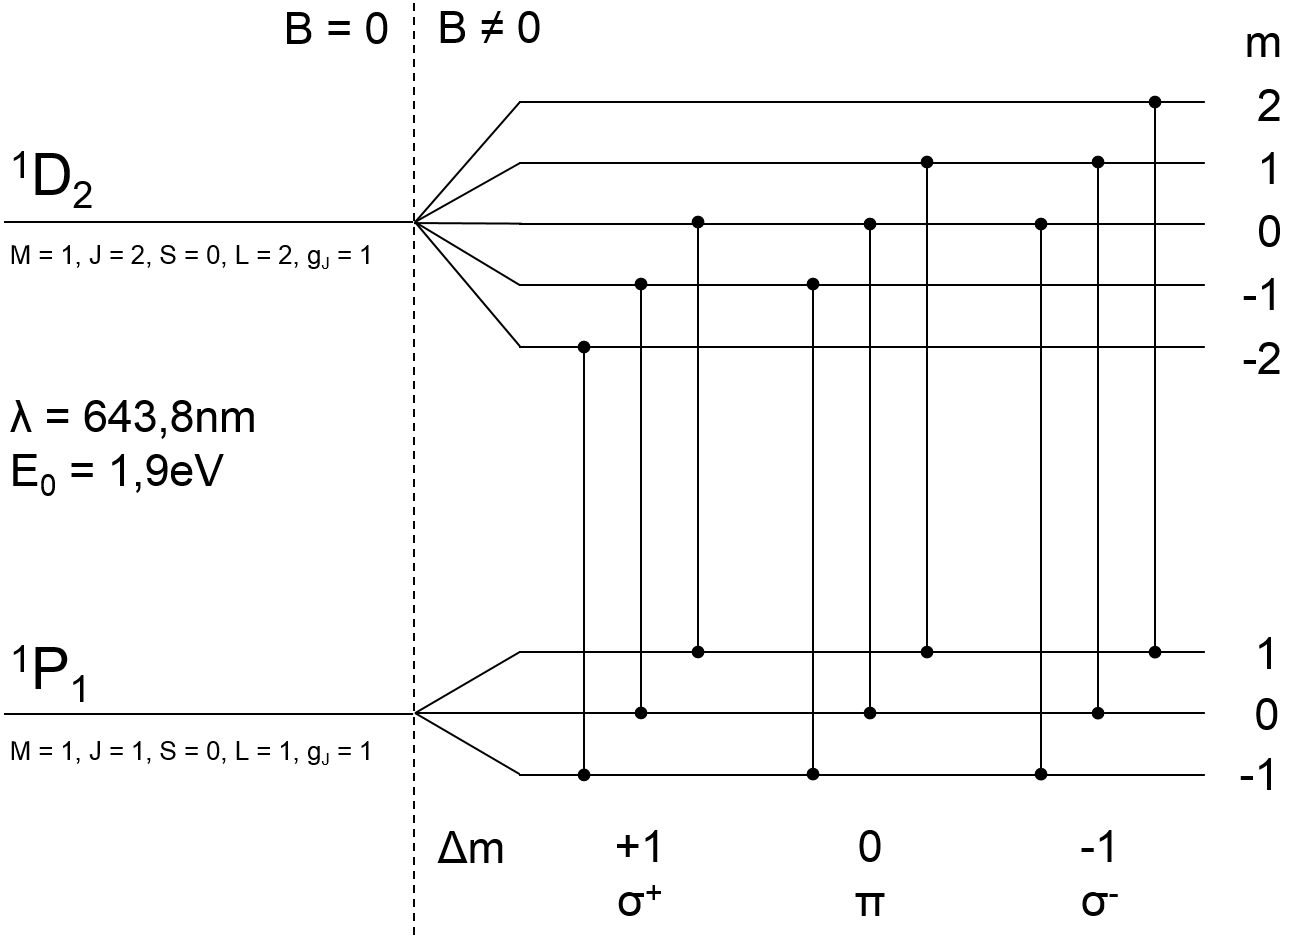
\includegraphics[width=0.8\textwidth]{img/rot}
	\caption{Termschema der roten Spektrallinie von Cadmium, normaler Zeeman-Effekt}
	\label{fig:rot}
\end{figure}
\begin{figure}
	\centering
	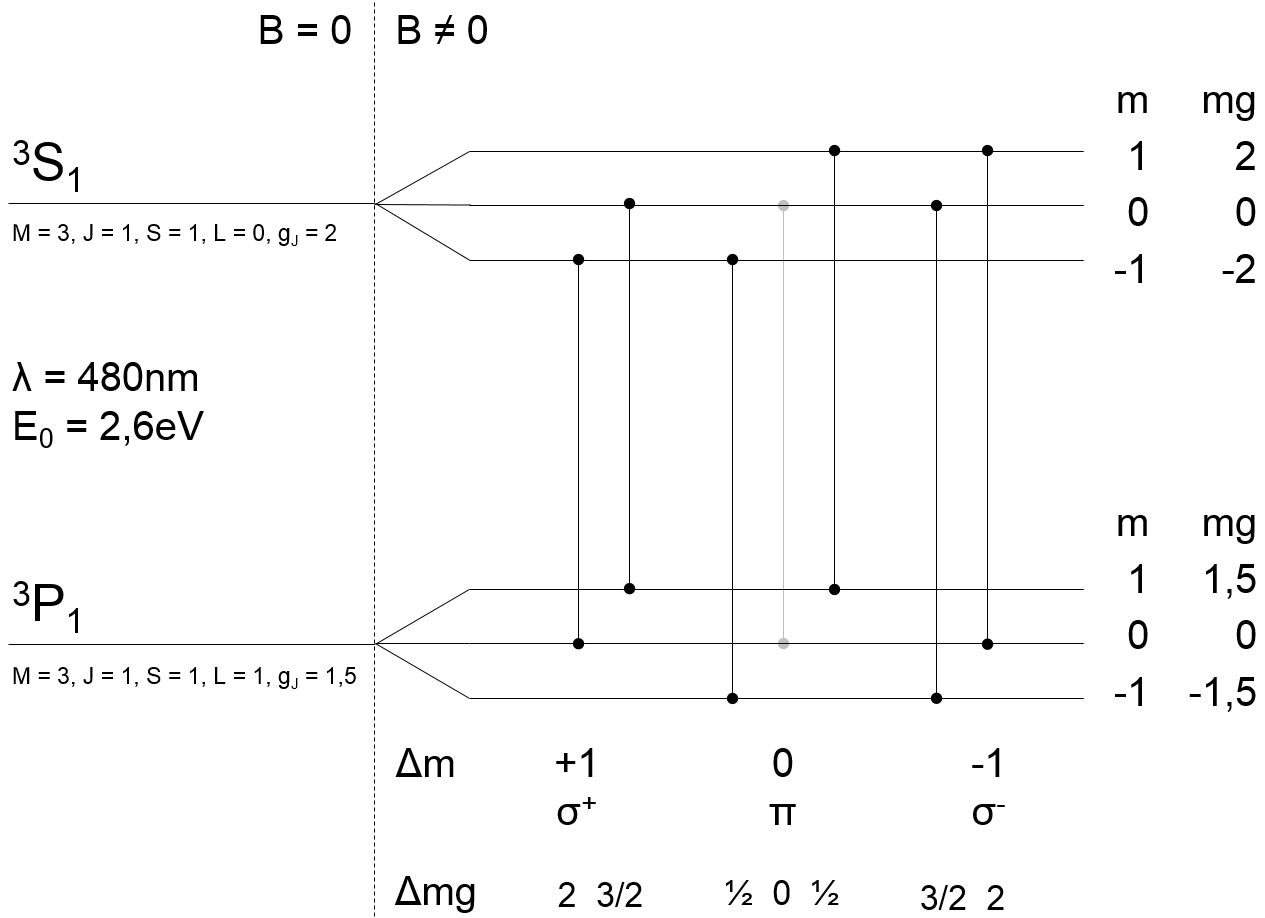
\includegraphics[width=0.8\textwidth]{img/blau}
	\caption{Termschema der blauen Spektrallinie von Cadmium, anormaler Zeeman-Effekt}
	\label{fig:blau}
\end{figure}

Die Abbildungen \ref{fig:rot} und \ref{fig:blau} zeigen das Termschema für die rote und blaue Linie des Cadmium-Spektrums, die in diesem Versuch untersucht werden sollen.
Bei der mittleren Linie der blauen Linie ($m_1 = m_2 = 0$) tritt ein Sonderfall auf, bei dem diese Linie nicht beobachtet wird, obwohl sie nach den oben beschriebenen Auswahlregeln erwartet wird.